\section{Cavity Domains}
  \subsection{Definition}
  A \textbf{cavity domain} is an open, path-connected set in which every point is further away from every atom than a given cutoff radius. The point in this set, which is furthest away from it's closest atom, is called the \textbf{cavity domain center}.
  
  \begin{figure}[h]
  \begin{center}
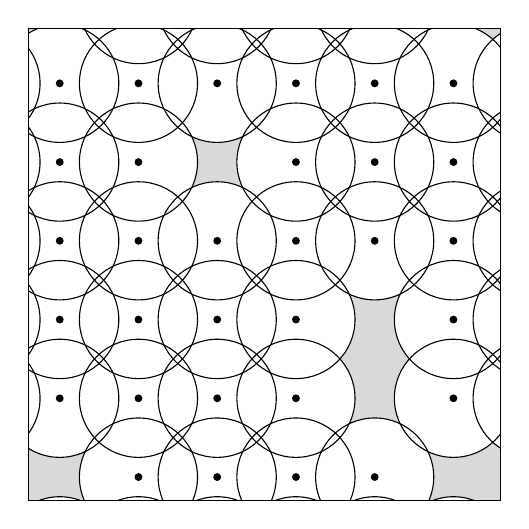
\begin{tikzpicture}
\fill[black!15!white] (0,0) rectangle (6,6);
\begin{scope}
\clip (0,0) rectangle (6,6);
\fill[white] (-1.600000,-1.700000) circle (0.75);
\fill[white] (-1.600000,-0.700000) circle (0.75);
\fill[white] (-1.600000,0.300000) circle (0.75);
\fill[white] (-1.600000,1.300000) circle (0.75);
\fill[white] (-1.600000,2.300000) circle (0.75);
\fill[white] (-1.600000,3.300000) circle (0.75);
\fill[white] (-1.600000,4.300000) circle (0.75);
\fill[white] (-1.600000,5.300000) circle (0.75);
\fill[white] (-1.600000,6.300000) circle (0.75);
\fill[white] (-1.600000,7.300000) circle (0.75);
\fill[white] (-1.600000,8.300000) circle (0.75);
\fill[white] (-0.600000,-1.700000) circle (0.75);
\fill[white] (-0.600000,-0.700000) circle (0.75);
%\fill[white] (-0.600000,0.300000) circle (0.75);
\fill[white] (-0.600000,1.300000) circle (0.75);
\fill[white] (-0.600000,2.300000) circle (0.75);
\fill[white] (-0.600000,3.300000) circle (0.75);
\fill[white] (-0.600000,4.300000) circle (0.75);
\fill[white] (-0.600000,5.300000) circle (0.75);
%\fill[white] (-0.600000,6.300000) circle (0.75);
\fill[white] (-0.600000,7.300000) circle (0.75);
\fill[white] (-0.600000,8.300000) circle (0.75);
\fill[white] (0.400000,-1.700000) circle (0.75);
\fill[white] (0.400000,-0.700000) circle (0.75);
%\fill[white] (0.400000,0.300000) circle (0.75);
\fill[white] (0.400000,1.300000) circle (0.75);
\fill[white] (0.400000,2.300000) circle (0.75);
\fill[white] (0.400000,3.300000) circle (0.75);
\fill[white] (0.400000,4.300000) circle (0.75);
\fill[white] (0.400000,5.300000) circle (0.75);
%\fill[white] (0.400000,6.300000) circle (0.75);
\fill[white] (0.400000,7.300000) circle (0.75);
\fill[white] (0.400000,8.300000) circle (0.75);
\fill[white] (1.400000,-1.700000) circle (0.75);
\fill[white] (1.400000,-0.700000) circle (0.75);
\fill[white] (1.400000,0.300000) circle (0.75);
\fill[white] (1.400000,1.300000) circle (0.75);
\fill[white] (1.400000,2.300000) circle (0.75);
\fill[white] (1.400000,3.300000) circle (0.75);
\fill[white] (1.400000,4.300000) circle (0.75);
\fill[white] (1.400000,5.300000) circle (0.75);
\fill[white] (1.400000,6.300000) circle (0.75);
\fill[white] (1.400000,7.300000) circle (0.75);
\fill[white] (1.400000,8.300000) circle (0.75);
\fill[white] (2.400000,-1.700000) circle (0.75);
\fill[white] (2.400000,-0.700000) circle (0.75);
\fill[white] (2.400000,0.300000) circle (0.75);
\fill[white] (2.400000,1.300000) circle (0.75);
\fill[white] (2.400000,2.300000) circle (0.75);
\fill[white] (2.400000,3.300000) circle (0.75);
%\fill[white] (2.400000,4.300000) circle (0.75);
\fill[white] (2.400000,5.300000) circle (0.75);
\fill[white] (2.400000,6.300000) circle (0.75);
\fill[white] (2.400000,7.300000) circle (0.75);
\fill[white] (2.400000,8.300000) circle (0.75);
\fill[white] (3.400000,-1.700000) circle (0.75);
\fill[white] (3.400000,-0.700000) circle (0.75);
\fill[white] (3.400000,0.300000) circle (0.75);
\fill[white] (3.400000,1.300000) circle (0.75);
\fill[white] (3.400000,2.300000) circle (0.75);
\fill[white] (3.400000,3.300000) circle (0.75);
\fill[white] (3.400000,4.300000) circle (0.75);
\fill[white] (3.400000,5.300000) circle (0.75);
\fill[white] (3.400000,6.300000) circle (0.75);
\fill[white] (3.400000,7.300000) circle (0.75);
\fill[white] (3.400000,8.300000) circle (0.75);
\fill[white] (4.400000,-1.700000) circle (0.75);
\fill[white] (4.400000,-0.700000) circle (0.75);
\fill[white] (4.400000,0.300000) circle (0.75);
%\fill[white] (4.400000,1.300000) circle (0.75);
%\fill[white] (4.400000,2.300000) circle (0.75);
\fill[white] (4.400000,3.300000) circle (0.75);
\fill[white] (4.400000,4.300000) circle (0.75);
\fill[white] (4.400000,5.300000) circle (0.75);
\fill[white] (4.400000,6.300000) circle (0.75);
\fill[white] (4.400000,7.300000) circle (0.75);
\fill[white] (4.400000,8.300000) circle (0.75);
\fill[white] (5.400000,-1.700000) circle (0.75);
\fill[white] (5.400000,-0.700000) circle (0.75);
%\fill[white] (5.400000,0.300000) circle (0.75);
\fill[white] (5.400000,1.300000) circle (0.75);
\fill[white] (5.400000,2.300000) circle (0.75);
\fill[white] (5.400000,3.300000) circle (0.75);
\fill[white] (5.400000,4.300000) circle (0.75);
\fill[white] (5.400000,5.300000) circle (0.75);
%\fill[white] (5.400000,6.300000) circle (0.75);
\fill[white] (5.400000,7.300000) circle (0.75);
\fill[white] (5.400000,8.300000) circle (0.75);
\fill[white] (6.400000,-1.700000) circle (0.75);
\fill[white] (6.400000,-0.700000) circle (0.75);
%\fill[white] (6.400000,0.300000) circle (0.75);
\fill[white] (6.400000,1.300000) circle (0.75);
\fill[white] (6.400000,2.300000) circle (0.75);
\fill[white] (6.400000,3.300000) circle (0.75);
\fill[white] (6.400000,4.300000) circle (0.75);
\fill[white] (6.400000,5.300000) circle (0.75);
%\fill[white] (6.400000,6.300000) circle (0.75);
\fill[white] (6.400000,7.300000) circle (0.75);
\fill[white] (6.400000,8.300000) circle (0.75);
\fill[white] (7.400000,-1.700000) circle (0.75);
\fill[white] (7.400000,-0.700000) circle (0.75);
\fill[white] (7.400000,0.300000) circle (0.75);
\fill[white] (7.400000,1.300000) circle (0.75);
\fill[white] (7.400000,2.300000) circle (0.75);
\fill[white] (7.400000,3.300000) circle (0.75);
\fill[white] (7.400000,4.300000) circle (0.75);
\fill[white] (7.400000,5.300000) circle (0.75);
\fill[white] (7.400000,6.300000) circle (0.75);
\fill[white] (7.400000,7.300000) circle (0.75);
\fill[white] (7.400000,8.300000) circle (0.75);
\fill[white] (8.400000,-1.700000) circle (0.75);
\fill[white] (8.400000,-0.700000) circle (0.75);
\fill[white] (8.400000,0.300000) circle (0.75);
\fill[white] (8.400000,1.300000) circle (0.75);
\fill[white] (8.400000,2.300000) circle (0.75);
\fill[white] (8.400000,3.300000) circle (0.75);
\fill[white] (8.400000,4.300000) circle (0.75);
\fill[white] (8.400000,5.300000) circle (0.75);
\fill[white] (8.400000,6.300000) circle (0.75);
\fill[white] (8.400000,7.300000) circle (0.75);
\fill[white] (8.400000,8.300000) circle (0.75);
\draw (-1.600000,-1.700000) circle (0.75);
\draw (-1.600000,-0.700000) circle (0.75);
\draw (-1.600000,0.300000) circle (0.75);
\draw (-1.600000,1.300000) circle (0.75);
\draw (-1.600000,2.300000) circle (0.75);
\draw (-1.600000,3.300000) circle (0.75);
\draw (-1.600000,4.300000) circle (0.75);
\draw (-1.600000,5.300000) circle (0.75);
\draw (-1.600000,6.300000) circle (0.75);
\draw (-1.600000,7.300000) circle (0.75);
\draw (-1.600000,8.300000) circle (0.75);
\draw (-0.600000,-1.700000) circle (0.75);
\draw (-0.600000,-0.700000) circle (0.75);
%\draw (-0.600000,0.300000) circle (0.75);
\draw (-0.600000,1.300000) circle (0.75);
\draw (-0.600000,2.300000) circle (0.75);
\draw (-0.600000,3.300000) circle (0.75);
\draw (-0.600000,4.300000) circle (0.75);
\draw (-0.600000,5.300000) circle (0.75);
%\draw (-0.600000,6.300000) circle (0.75);
\draw (-0.600000,7.300000) circle (0.75);
\draw (-0.600000,8.300000) circle (0.75);
\draw (0.400000,-1.700000) circle (0.75);
\draw (0.400000,-0.700000) circle (0.75);
%\draw (0.400000,0.300000) circle (0.75);
\draw (0.400000,1.300000) circle (0.75);
\draw (0.400000,2.300000) circle (0.75);
\draw (0.400000,3.300000) circle (0.75);
\draw (0.400000,4.300000) circle (0.75);
\draw (0.400000,5.300000) circle (0.75);
%\draw (0.400000,6.300000) circle (0.75);
\draw (0.400000,7.300000) circle (0.75);
\draw (0.400000,8.300000) circle (0.75);
\draw (1.400000,-1.700000) circle (0.75);
\draw (1.400000,-0.700000) circle (0.75);
\draw (1.400000,0.300000) circle (0.75);
\draw (1.400000,1.300000) circle (0.75);
\draw (1.400000,2.300000) circle (0.75);
\draw (1.400000,3.300000) circle (0.75);
\draw (1.400000,4.300000) circle (0.75);
\draw (1.400000,5.300000) circle (0.75);
\draw (1.400000,6.300000) circle (0.75);
\draw (1.400000,7.300000) circle (0.75);
\draw (1.400000,8.300000) circle (0.75);
\draw (2.400000,-1.700000) circle (0.75);
\draw (2.400000,-0.700000) circle (0.75);
\draw (2.400000,0.300000) circle (0.75);
\draw (2.400000,1.300000) circle (0.75);
\draw (2.400000,2.300000) circle (0.75);
\draw (2.400000,3.300000) circle (0.75);
%\draw (2.400000,4.300000) circle (0.75);
\draw (2.400000,5.300000) circle (0.75);
\draw (2.400000,6.300000) circle (0.75);
\draw (2.400000,7.300000) circle (0.75);
\draw (2.400000,8.300000) circle (0.75);
\draw (3.400000,-1.700000) circle (0.75);
\draw (3.400000,-0.700000) circle (0.75);
\draw (3.400000,0.300000) circle (0.75);
\draw (3.400000,1.300000) circle (0.75);
\draw (3.400000,2.300000) circle (0.75);
\draw (3.400000,3.300000) circle (0.75);
\draw (3.400000,4.300000) circle (0.75);
\draw (3.400000,5.300000) circle (0.75);
\draw (3.400000,6.300000) circle (0.75);
\draw (3.400000,7.300000) circle (0.75);
\draw (3.400000,8.300000) circle (0.75);
\draw (4.400000,-1.700000) circle (0.75);
\draw (4.400000,-0.700000) circle (0.75);
\draw (4.400000,0.300000) circle (0.75);
%\draw (4.400000,1.300000) circle (0.75);
%\draw (4.400000,2.300000) circle (0.75);
\draw (4.400000,3.300000) circle (0.75);
\draw (4.400000,4.300000) circle (0.75);
\draw (4.400000,5.300000) circle (0.75);
\draw (4.400000,6.300000) circle (0.75);
\draw (4.400000,7.300000) circle (0.75);
\draw (4.400000,8.300000) circle (0.75);
\draw (5.400000,-1.700000) circle (0.75);
\draw (5.400000,-0.700000) circle (0.75);
%\draw (5.400000,0.300000) circle (0.75);
\draw (5.400000,1.300000) circle (0.75);
\draw (5.400000,2.300000) circle (0.75);
\draw (5.400000,3.300000) circle (0.75);
\draw (5.400000,4.300000) circle (0.75);
\draw (5.400000,5.300000) circle (0.75);
%\draw (5.400000,6.300000) circle (0.75);
\draw (5.400000,7.300000) circle (0.75);
\draw (5.400000,8.300000) circle (0.75);
\draw (6.400000,-1.700000) circle (0.75);
\draw (6.400000,-0.700000) circle (0.75);
%\draw (6.400000,0.300000) circle (0.75);
\draw (6.400000,1.300000) circle (0.75);
\draw (6.400000,2.300000) circle (0.75);
\draw (6.400000,3.300000) circle (0.75);
\draw (6.400000,4.300000) circle (0.75);
\draw (6.400000,5.300000) circle (0.75);
%\draw (6.400000,6.300000) circle (0.75);
\draw (6.400000,7.300000) circle (0.75);
\draw (6.400000,8.300000) circle (0.75);
\draw (7.400000,-1.700000) circle (0.75);
\draw (7.400000,-0.700000) circle (0.75);
\draw (7.400000,0.300000) circle (0.75);
\draw (7.400000,1.300000) circle (0.75);
\draw (7.400000,2.300000) circle (0.75);
\draw (7.400000,3.300000) circle (0.75);
\draw (7.400000,4.300000) circle (0.75);
\draw (7.400000,5.300000) circle (0.75);
\draw (7.400000,6.300000) circle (0.75);
\draw (7.400000,7.300000) circle (0.75);
\draw (7.400000,8.300000) circle (0.75);
\draw (8.400000,-1.700000) circle (0.75);
\draw (8.400000,-0.700000) circle (0.75);
\draw (8.400000,0.300000) circle (0.75);
\draw (8.400000,1.300000) circle (0.75);
\draw (8.400000,2.300000) circle (0.75);
\draw (8.400000,3.300000) circle (0.75);
\draw (8.400000,4.300000) circle (0.75);
\draw (8.400000,5.300000) circle (0.75);
\draw (8.400000,6.300000) circle (0.75);
\draw (8.400000,7.300000) circle (0.75);
\draw (8.400000,8.300000) circle (0.75);
\fill (-1.600000,-1.700000) circle (0.05);
\fill (-1.600000,-0.700000) circle (0.05);
\fill (-1.600000,0.300000) circle (0.05);
\fill (-1.600000,1.300000) circle (0.05);
\fill (-1.600000,2.300000) circle (0.05);
\fill (-1.600000,3.300000) circle (0.05);
\fill (-1.600000,4.300000) circle (0.05);
\fill (-1.600000,5.300000) circle (0.05);
\fill (-1.600000,6.300000) circle (0.05);
\fill (-1.600000,7.300000) circle (0.05);
\fill (-1.600000,8.300000) circle (0.05);
\fill (-0.600000,-1.700000) circle (0.05);
\fill (-0.600000,-0.700000) circle (0.05);
\fill (-0.600000,0.300000) circle (0.05);
\fill (-0.600000,1.300000) circle (0.05);
\fill (-0.600000,2.300000) circle (0.05);
\fill (-0.600000,3.300000) circle (0.05);
\fill (-0.600000,4.300000) circle (0.05);
\fill (-0.600000,5.300000) circle (0.05);
\fill (-0.600000,6.300000) circle (0.05);
\fill (-0.600000,7.300000) circle (0.05);
\fill (-0.600000,8.300000) circle (0.05);
\fill (0.400000,-1.700000) circle (0.05);
\fill (0.400000,-0.700000) circle (0.05);
%\fill (0.400000,0.300000) circle (0.05);
\fill (0.400000,1.300000) circle (0.05);
\fill (0.400000,2.300000) circle (0.05);
\fill (0.400000,3.300000) circle (0.05);
\fill (0.400000,4.300000) circle (0.05);
\fill (0.400000,5.300000) circle (0.05);
\fill (0.400000,6.300000) circle (0.05);
\fill (0.400000,7.300000) circle (0.05);
\fill (0.400000,8.300000) circle (0.05);
\fill (1.400000,-1.700000) circle (0.05);
\fill (1.400000,-0.700000) circle (0.05);
\fill (1.400000,0.300000) circle (0.05);
\fill (1.400000,1.300000) circle (0.05);
\fill (1.400000,2.300000) circle (0.05);
\fill (1.400000,3.300000) circle (0.05);
\fill (1.400000,4.300000) circle (0.05);
\fill (1.400000,5.300000) circle (0.05);
\fill (1.400000,6.300000) circle (0.05);
\fill (1.400000,7.300000) circle (0.05);
\fill (1.400000,8.300000) circle (0.05);
\fill (2.400000,-1.700000) circle (0.05);
\fill (2.400000,-0.700000) circle (0.05);
\fill (2.400000,0.300000) circle (0.05);
\fill (2.400000,1.300000) circle (0.05);
\fill (2.400000,2.300000) circle (0.05);
\fill (2.400000,3.300000) circle (0.05);
%\fill (2.400000,4.300000) circle (0.05);
\fill (2.400000,5.300000) circle (0.05);
\fill (2.400000,6.300000) circle (0.05);
\fill (2.400000,7.300000) circle (0.05);
\fill (2.400000,8.300000) circle (0.05);
\fill (3.400000,-1.700000) circle (0.05);
\fill (3.400000,-0.700000) circle (0.05);
\fill (3.400000,0.300000) circle (0.05);
\fill (3.400000,1.300000) circle (0.05);
\fill (3.400000,2.300000) circle (0.05);
\fill (3.400000,3.300000) circle (0.05);
\fill (3.400000,4.300000) circle (0.05);
\fill (3.400000,5.300000) circle (0.05);
\fill (3.400000,6.300000) circle (0.05);
\fill (3.400000,7.300000) circle (0.05);
\fill (3.400000,8.300000) circle (0.05);
\fill (4.400000,-1.700000) circle (0.05);
\fill (4.400000,-0.700000) circle (0.05);
\fill (4.400000,0.300000) circle (0.05);
%\fill (4.400000,1.300000) circle (0.05);
%\fill (4.400000,2.300000) circle (0.05);
\fill (4.400000,3.300000) circle (0.05);
\fill (4.400000,4.300000) circle (0.05);
\fill (4.400000,5.300000) circle (0.05);
\fill (4.400000,6.300000) circle (0.05);
\fill (4.400000,7.300000) circle (0.05);
\fill (4.400000,8.300000) circle (0.05);
\fill (5.400000,-1.700000) circle (0.05);
\fill (5.400000,-0.700000) circle (0.05);
%\fill (5.400000,0.300000) circle (0.05);
\fill (5.400000,1.300000) circle (0.05);
\fill (5.400000,2.300000) circle (0.05);
\fill (5.400000,3.300000) circle (0.05);
\fill (5.400000,4.300000) circle (0.05);
\fill (5.400000,5.300000) circle (0.05);
\fill (5.400000,6.300000) circle (0.05);
\fill (5.400000,7.300000) circle (0.05);
\fill (5.400000,8.300000) circle (0.05);
\fill (6.400000,-1.700000) circle (0.05);
\fill (6.400000,-0.700000) circle (0.05);
\fill (6.400000,0.300000) circle (0.05);
\fill (6.400000,1.300000) circle (0.05);
\fill (6.400000,2.300000) circle (0.05);
\fill (6.400000,3.300000) circle (0.05);
\fill (6.400000,4.300000) circle (0.05);
\fill (6.400000,5.300000) circle (0.05);
\fill (6.400000,6.300000) circle (0.05);
\fill (6.400000,7.300000) circle (0.05);
\fill (6.400000,8.300000) circle (0.05);
\fill (7.400000,-1.700000) circle (0.05);
\fill (7.400000,-0.700000) circle (0.05);
\fill (7.400000,0.300000) circle (0.05);
\fill (7.400000,1.300000) circle (0.05);
\fill (7.400000,2.300000) circle (0.05);
\fill (7.400000,3.300000) circle (0.05);
\fill (7.400000,4.300000) circle (0.05);
\fill (7.400000,5.300000) circle (0.05);
\fill (7.400000,6.300000) circle (0.05);
\fill (7.400000,7.300000) circle (0.05);
\fill (7.400000,8.300000) circle (0.05);
\fill (8.400000,-1.700000) circle (0.05);
\fill (8.400000,-0.700000) circle (0.05);
\fill (8.400000,0.300000) circle (0.05);
\fill (8.400000,1.300000) circle (0.05);
\fill (8.400000,2.300000) circle (0.05);
\fill (8.400000,3.300000) circle (0.05);
\fill (8.400000,4.300000) circle (0.05);
\fill (8.400000,5.300000) circle (0.05);
\fill (8.400000,6.300000) circle (0.05);
\fill (8.400000,7.300000) circle (0.05);
\fill (8.400000,8.300000) circle (0.05);
\end{scope}
\draw (0,0) rectangle (6,6);
\end{tikzpicture}
\end{center}
\caption{Cavity domains in a cubic crystal structure with missing atoms (x-y-plane)}
\end{figure}
  %------------
  \subsection{Input data}
  The following values must be provided to find cavity domains:
  \begin{description}
    \item[$\mathcal{V}(\mathcal{X})$] The \textbf{analyzed volume}.
    \item[$v_1, v_2, v_3$] The \textbf{translation vectors}.
    \item[$p_i$] The \textbf{atom positions} in $\mathcal{V}(\mathcal{B})$, with $p_{i,j}$ being the $j$-th component of the $i$-th atom's position. $n$ is the number of atoms.
    \item[$r_i$] The atom \textbf{cutoff radii}.
  \end{description}
  %------------
  \subsection{Finding Cavity Domains in Continuous Space}
  \begin{enumerate}
  \item{Define a function $g(x)$ which maps each point $x$ to the index of the \emph{any} atom position with a distance to $x$ less than or equal to the atom's cutoff radius, or 0 if no such atom exists.
  \[G(x) = \{i|~ |p_{i}-x| \le r_i,i \in \mathbb{N}^{\le n}\}\]
  \[g(x) = \left\{\begin{array}{ll}\hat{g} \in G(x)&\text{if } G(x) \ne \varnothing\\0&\text{otherwise}\end{array}\right.\]
  Note: $g(x) = 0 \Leftrightarrow G(x) = \varnothing \Leftrightarrow$ The point $x$ is part of a cavity domain.}
  \item{Now each open, non-empty set $S_i \subseteq \mathcal{V}(\mathcal{B})$ which meets the following conditions is a cavity domain:
  \begin{itemize}
  \item{All points in $S_i$ are part of a cavity domain:
  \[\forall x \in S_i\colon g(x) = 0\]}
  \item{$S_i$ is path-connected:
  \[\forall x, y \in S_i\colon \exists f(t) \in C(S_i)\colon f(0) = x, f(1) = y, f(t) \in S_i ~ \forall 0 \le t \le 1\]}
  \item{No limit point of $S_i$ is inside of a cavity domain:
  \[\forall y \in \partial{S_i}\colon g(y) \ne 0 \]
  Note: This means that $S_i$ includes as many points as possible without violating any prior condition.}
  \end{itemize}}
  \item{For each cavity domain $S_i$ the center $c_i$ is defined as the point with the greatest distance to the closest atom:
  \[c_i\colon \min_{p_i}(|c_i-p_i|) \ge \min_{p_i}(|x-p_i|) \forall x \in S_i\]
  }
  \end{enumerate}
  %------------
  


\subsection{Finding Cavity Domain Approximations in Discrete Space}

In this section, the cavity domains are approximated by defining them on the set of discretization points $\mathcal{D}$ and using approximations for the atom positions.
\begin{enumerate}
\item {The atom positions $p_i$ are approximated by points $\tilde{p}_i \in \mathcal{V}(\mathcal{D})$:
\[|\tilde{p}_{i}-p_{i}| = \min_{x \in \mathcal{V}(\mathcal{D})}(|x-p_{i}|)\]
}
\item {The definition of $\tilde{g}(x)\colon \mathcal{D} \rightarrow \mathbb{N}_0$ is the almost the same as the one in the last section, but instead of the atom positions $p_i$, their approximations $\tilde{p}_j$ are used:
\[\tilde{G}(x) = \{i|~ |\tilde{p}_{i}-x| \le r_i,i \in \mathbb{N}^{\le n}\}\]
  \[\tilde{g}(x) = \left\{\begin{array}{ll}\hat{g} \in \tilde{G}(x)&\text{if } \tilde{G}(x) \ne \varnothing\\0&\text{otherwise}\end{array}\right.\]
}
\item Each non-empty set $\tilde{S}_i \subseteq \mathcal{V}(\mathcal{D})$ which meets the following conditions is a cavity domain approximation:
\begin{itemize}
  \item{All points in $\tilde{S}_i$ are part of a cavity domain:
  \[\forall x \in \tilde{S}_i\colon \tilde{g}(x) = 0\]}
\item{Every point $x$ in $\tilde{S}_i$ can be reached from every point $y$ in $\tilde{S}_i$ by a series of "neighbor" points $c_j$ that are also inside of $\tilde{S}_i$:
\[
\forall x \in \tilde{S}_i, \forall y \in \tilde{S}_i,\exists c_j \in \tilde{S}_i\colon c_0 = x, c_m = y,|c_{j+1}-c_j| \le \sqrt{3}*s_{step}
\]
}
\item{No "neighbor" point of $\tilde{S}_i$ is also part of a cavity domain:
\[
\forall x \in \tilde{S}_i, \forall y \in \mathcal{V}(\mathcal{D})\colon |x-y| > \sqrt{3}*s_{step}  \lor \tilde{g}(y)\ne0  \lor y \in \tilde{S}_i
\]
}
\end{itemize}
\item{
Cavity domain approximation centers are defined like cavity domain centers as the points with the greatest distance to the closest atom:

  \[\tilde{s}_i\colon \min_{p_i}(|\tilde{c}_i-p_i|) \ge \min_{p_i}(|x-p_i|) \forall x \in \tilde{S}_i\]
}
\end{enumerate}



  \subsection{Algorithm}
  \label{domainalgorithm}
For the purpose of implementing this approximation, a bijective mapping between $\mathcal{Z}=([0,d_1-1] \times [0,d_2-1]\times [0,d_3-1]) \cap \mathbb{N}_0^3$ and $\mathcal{D}$ is defined:
\begin{align*}
o &= \min_{y \in \mathcal{D}}(y_1+y_2+y_3) \in \mathcal{D}\\
T(x) &= o+x\cdot s_{step} \in \mathcal{D} ~\forall x\in\mathcal{Z}\\
\Leftrightarrow T^{-1}(x) &= \frac{x-o}{s_{step}} \in \mathcal{Z} ~\forall x\in\mathcal{D}\\
\end{align*}
Whenever an implementation uses zero-based three-dimensional indices instead of points in $\mathcal{D}$, this mapping can be used.
\begin{enumerate}
\item{Approximated translation vectors are calculated as described earlier, so that $\forall x \in \mathcal{D}\colon \exists n\in\mathbb{Z}^3\colon x+\sum_{i=1}^3 \tilde{v}_i \cdot n_i \in \mathcal{V}(\mathcal{D})$:

\[
\tilde{v}_{i,j} = \begin{cases}0 & \text{if } v_{i,j} = 0\\
2 s_{step}\left\lfloor \frac{1}{2} \frac{v_{i,j}}{s_{step}}\right\rfloor + (d_i \bmod 2) s_{step}& \text{otherwise}\end{cases}
\]
}
\item{The approximated atom positions are calculated:
\begin{align*}
\hat{p}_{i,j} &= \left\lfloor\frac{p_{i,j}}{s_{step}}+0.5\right\rfloor \cdot s_{step} ~\forall j \in [1,3]\\
\tilde{p}_i &= \hat{p}_i+ \sum_{i=1}^3 \tilde{v}_i \cdot n_i,~ n \in \mathbb{Z}^3,~ \tilde{p}_i \in \mathcal{V(\mathcal{D})}\\
\end{align*}
}
\item{$g(x)$ is implemented as a three-dimensional array of signed (for later use of the negative range) integers. Instead of filling it cell-by-cell, it is first initialized to 0 and then filled atom-by-atom. For each atom the following actions are performed:
\begin{enumerate}
\item {\[\tilde{r}_i = \left\lfloor \frac{r_i}{s_{step}} +0.5 \right\rfloor\]}
\item {Create a three-dimensional array $m$ with indices in $[0,2\tilde{r}_i]^3$:
\[m[j,k,l] = \left\{\begin{array}{cl}i&\text{if }(j-\tilde{r}_i)^2+(k-\tilde{r}_i)^2+(l-\tilde{r}_i)^2 < r_i^2\\0&\text{otherwise}\end{array}\right.\]}
\item {For each $j$ in $[0,2\tilde{r}_i]^3$:\\
For each $k$ in $\{-1,0,1\}^3$:\\
\begin{align*}
x &= \tilde{p}_i + \sum_{l=1}^3 \tilde{v}_l \cdot k_l + j-\tilde{r}_i\\
g[x_1,x_2,x_3] &\leftarrow m[j_1,j_2,j_3]
\end{align*}
}
\end{enumerate}
This approach is chosen so that the same $m$ can be used for all atoms of the same element.
}
\item{In this last step, the cavity domains are "built" from the points $x$ with $g[x_1,x_2,x_3] = 0$. At the same time, cavity centers are found. This is shown in the following pseudocode:

\begin{algorithmic}
\State $i\gets 0$
\ForAll{$x \in \mathcal{Z}$}
    \If {$g[x_1,x_2,x_3] = 0$}
        \State $i \gets i+1$
        \State $maxdist \gets -1$
        \State $maxdistpoint \gets x$
        \State $neighbors \gets$ new stack
        \State Push $x$ to $neighbors$
        \While{$neighbors$ is not empty}
            \State $y \gets neighbors.pop()$
            \If{$g[y_1,y_2,y_3] = 0$}
                \State $g[y_1,y_2,y_3] = -i$
                \State $dist = \min(|\tilde{p}_i - y|)$
                \If{($maxdist = -1$) or ($maxdist > dist$)}
                    \State $maxdist \gets dist$
                    \State $maxdistpoint \gets y$
                \EndIf
                \State Push neighbors of $y$ to $neighbors$
            \EndIf
        \EndWhile
        \State $centers[i-1] \gets maxdistpoint$
    \EndIf
\EndFor
\State $numberofcavities \gets i$
\end{algorithmic}





}
\end{enumerate}
